\documentclass{article}
\usepackage[utf8]{inputenc}
\usepackage{geometry}
 \geometry{
 a4paper,
 total={170mm,257mm},
 left=20mm,
 top=20mm,
 }
 \usepackage{graphicx}
 \usepackage{titling}
 \usepackage{hyperref} 
 \usepackage{sourcecodepro} 
 \usepackage{tabularx} 
 \usepackage{amssymb}

 \title{Computer Networks\\ Assignment 1
}
\author{Jaskirat Singh Maskeen (23110146) \&  Karan Sagar Gandhi (23110157)}
\date{September 9, 2025}
 
 \usepackage{fancyhdr}
\fancypagestyle{plain}{
    \fancyhf{} 
    \fancyfoot[L]{\thedate}
    \fancyhead[L]{DNS and Traceroute}
    \fancyhead[R]{\theauthor}
}
\makeatletter
\def\@maketitle{%
  \newpage
  \null
  \vskip 1em%
  \begin{center}%
  \let \footnote \thanks
    {\LARGE \@title \par}%
    \vskip 1em%
  \end{center}%
  \par
  \vskip 1em}
\makeatother

\usepackage{lipsum}  
\usepackage{cmbright}

\begin{document}

\maketitle

\noindent\begin{tabular}{@{}ll}
    Students & \theauthor\\
    Professor &  Sameer G. Kulkarni
\end{tabular}

\section{DNS Resolver}

The objective of this task was to develop a custom DNS resolution system. The system consists of a client that parses DNS queries from a PCAP file and a server that resolves these queries based on a set of custom rules.

\subsection{System Architecture and Flow}

The operational flow of the system is as follows:
\begin{enumerate}
    \item \textbf{Packet Filtering:} The client begins by reading a given \texttt{.pcap} file and filtering it to isolate the DNS query packets (these are the queries which are sent to UDP port 53).
    \item \textbf{Custom Header Addition:} For each DNS query, the client generates an 8-byte custom header with the format \texttt{"HHMMSSID"}. This header contains the current time and a two-digit sequence ID for the query (The sequence ID is incremented after each query).
    \item \textbf{Communication:} The client sends the original DNS query, prefixed with this custom header, to the server.
    \item \textbf{Server-Side Processing:} The server receives the message, parses the custom header to determine the appropriate IP pool based on the timestamp, and extracts the domain name from the DNS query payload (following~\cite{rfc1035}).
    \item \textbf{Response and Logging:} The server sends the resolved IP address, the domain name, and the original custom header back to the client. The client then logs this information. To better simulate real-world conditions, we allow the client introduces an artificial delay (random, configurable) between sending DNS queries.
\end{enumerate}

\subsection{Transport Protocol: TCP to UDP}

\subsubsection{Initial TCP Implementation}
Our initial implementation for the client-server communication was built using TCP (\texttt{SOCK\_STREAM}). However, TCP being a stream protocol, without message boundaries, we had to implement our own mechanism to identify the start of the message. This was done by prefixing each payload with a 4-byte unsigned integer which represents the payload's length. The receiver (client or server) would first read these 4 bytes to determine the message size and then read that exact number of bytes to get the complete message.

\subsubsection{Current UDP Implementation}
After a discussion with the professor, we decided to use UDP (\texttt{SOCK\_DGRAM}) as our communication protocol. This change was motivated by the fact that real-world DNS queries majorly use UDP due to its low overhead (No handshakes, unlike TCP). However it is to be noted that incase size of the message is more than 512 bytes, TCP will be used~\cite{rfc1035}, but we stick to UDP in our implementation.  

UDP is a message-oriented protocol, meaning it preserves message boundaries automatically. Hence this allowed us to remove the manual 4-byte length prefixing, simplifying our message handling logic. 

\subsection{Implementation Details}
\begin{itemize}
    \item \texttt{3.pcap}: The pcap file from where we process the DNS queries. ($ 23110146 + 23110157 \equiv 3 \pmod{10} $)
    \item \texttt{client.py}: Manages reading the PCAP file, sending queries, and displaying results.
    \item \texttt{server.py}: Listens for incoming queries, applies the routing logic, and sends back responses.
    \item \texttt{helpers.py}: Contains utility functions for DNS packet parsing, including logic to handle domain name decompression as specified in~\cite{rfc1035}.
    \item \texttt{rules.json}: An external configuration file that defines the time-based routing rules, allowing for easy modification without changing the server code.
\end{itemize}

\subsection{Results}
The client successfully processed the DNS queries from \texttt{3.pcap} and received the resolved IP addresses from the server. The final output is shown in the table below.
Note that we ran this at \texttt{Tuesday 09/09/2025 22:32:20}.

\begin{center}
\begin{tabularx}{\textwidth}{|l|X|l|}
\hline
\textbf{Custom Header} & \textbf{Domain} & \textbf{Resolved IP Address} \\
\hline
\texttt{22322400} & \texttt{netflix.com} & \texttt{192.168.1.11} \\
\hline
\texttt{22322801} & \texttt{linkedin.com} & \texttt{192.168.1.12} \\
\hline
\texttt{22323202} & \texttt{example.com} & \texttt{192.168.1.13} \\
\hline
\texttt{22323303} & \texttt{google.com} & \texttt{192.168.1.14} \\
\hline
\texttt{22323704} & \texttt{facebook.com} & \texttt{192.168.1.15} \\
\hline
\texttt{22324205} & \texttt{amazon.com} & \texttt{192.168.1.11} \\
\hline
\end{tabularx}
\end{center}

\begin{figure}[H]
    \centering
    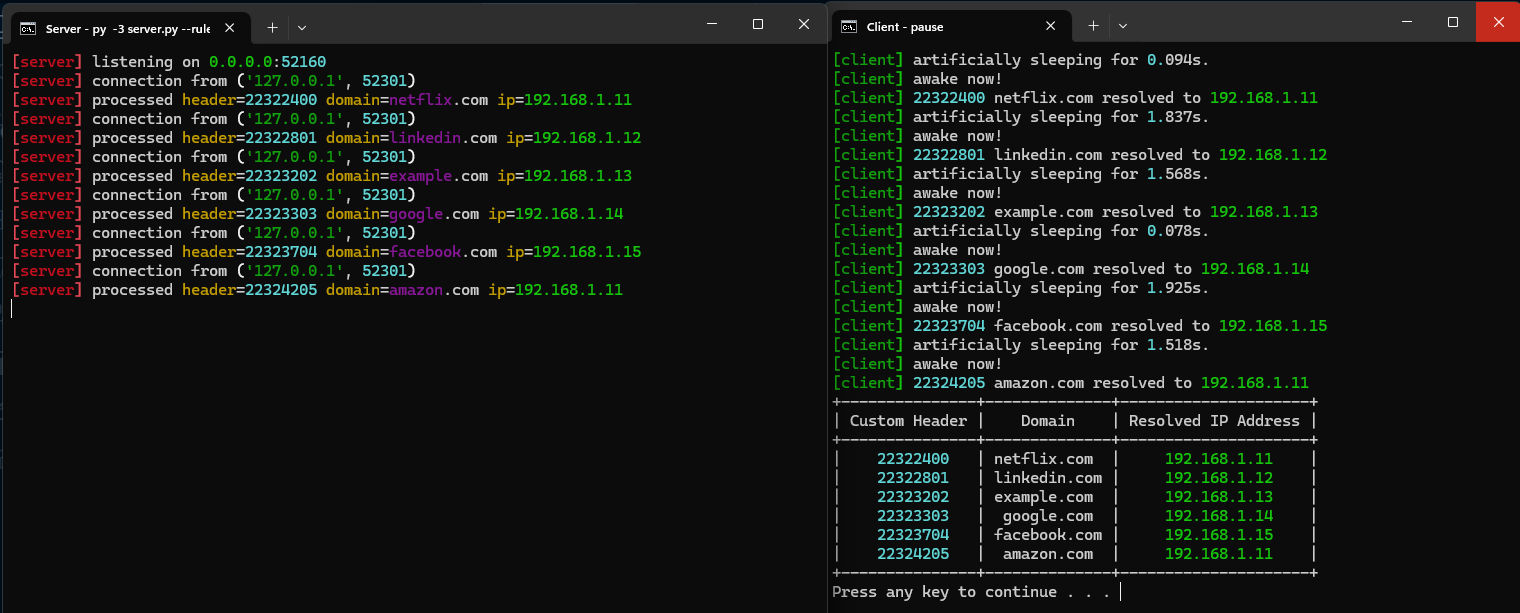
\includegraphics[width=\textwidth]{task1.png}
    \caption{Screenshot of the client and server running.}
\end{figure}

\subsection{Important sections refered in~\cite{rfc1035}}
\begin{enumerate}
\item 4.1.1. Header section format
\item 4.1.2. Question section format 
\item 4.1.4. Message compression  
\end{enumerate}

\bibliographystyle{plain}
\bibliography{references}

\end{document}